% Created 2018-01-31 三 11:09
% Intended LaTeX compiler: pdflatex
\documentclass[UTF8]{ctexart}
\usepackage{titlesec}
\usepackage{hyperref}

\usepackage[Lenny]{fncychap}
\usepackage[figuresright]{rotating}
\usepackage{capt-of}
\usepackage{amssymb}
\usepackage[normalem]{ulem}
\usepackage{wrapfig}
\usepackage{grffile}
\usepackage{booktabs}
\usepackage{tabularx}
\usepackage{amsmath}
\usepackage{textcomp}
\usepackage{fancyhdr}
\usepackage{tikz}
\usepackage{longtable}
\usepackage{float}
\usepackage{geometry}
\usepackage{xunicode}
\usepackage{indentfirst}
\usepackage{fontspec}
\usepackage{listings}
\usepackage{xcolor}

\parindent 2em

\setCJKmainfont{WenQuanYi Micro Hei} % 设置缺省中文字体
\setCJKsansfont{WenQuanYi Micro Hei}
\setCJKmonofont{WenQuanYi Micro Hei Mono}

\setmainfont{DejaVu Sans} % 英文衬线字体
\setsansfont{DejaVu Serif} % 英文无衬线字体
\setmonofont{DejaVu Sans Mono}
%\setmainfont{WenQuanYi Micro Hei} % 设置缺省中文字体
%\setsansfont{WenQuanYi Micro Hei}
%\setmonofont{WenQuanYi Micro Hei Mono}

%如果没有它,会有一些 tex 特殊字符无法正常使用,比如连字符。
\defaultfontfeatures{Mapping=tex-text}

% 中文断行
\XeTeXlinebreaklocale "zh"
\XeTeXlinebreakskip = 0pt plus 1pt minus 0.1pt

% 代码设置
\lstset{numbers=left,
numberstyle= \tiny,
keywordstyle= \color{ blue!70},commentstyle=\color{red!50!green!50!blue!50},
frame=shadowbox,
breaklines=true,
rulesepcolor= \color{ red!20!green!20!blue!20}
}
\author{jacksoncy}
\date{\today}
\title{协程调度}
\hypersetup{
 pdfauthor={jacksoncy},
 pdftitle={协程调度},
 pdfkeywords={},
 pdfsubject={},
 pdfcreator={Emacs 25.3.1 (Org mode 9.1.6)}, 
 pdflang={English}}
\begin{document}

\maketitle
\tableofcontents


\section{简单科普}
\label{sec:orgd3959ca}
\subsubsection{并发与并行}
\label{sec:org44588fa}
\begin{center}
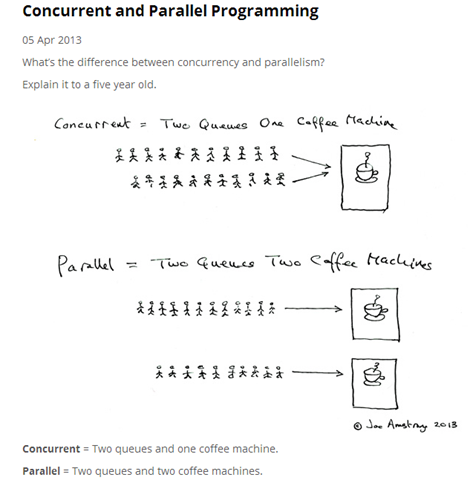
\includegraphics[width=.9\linewidth]{./parallelism.png}
\end{center}

并发讲究的是任务的切分(就如 \texttt{Nginx} 里将一个完整的 \texttt{HTTP} 请求拆分成 11 个任务片段),提高系统并发量。

并行是同时执行任务,提高系统的吞吐量(前提必须是硬件的多核)。
\subsubsection{硬件并行架构}
\label{sec:org4a77e3c}
摩尔定律:积体电路上可容纳的电晶体(晶体管)数目,约每隔两年便会增加一倍。

近年来随着摩尔定律的失效,各 \texttt{CPU} 厂商开始多核心架构设计进而带动软件的并行化。

一个典型的芯片多线程、多核、多处理器系统,如下图:

\begin{center}
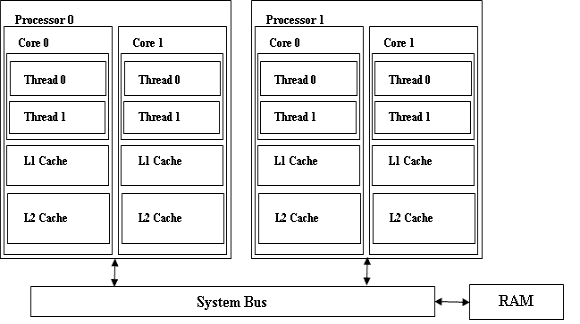
\includegraphics[width=.9\linewidth]{./multicore_mp_system.png}
\end{center}
\subsubsection{协程与线程}
\label{sec:org25ffeb8}
进程是程序的基本执行实体,线程是独立调度和分派的基本单位。

协程最初在 1963 年被公开提出(PS:这个比进程概念要早)。

对于进程、线程,都是由内核进行调度,有 \texttt{CPU} 时间片的概念,进行 \textbf{抢占式调度} (当然还有其他多种调度算法,毕竟线程调度是操作系统非常复杂的一部分)。

    对于协程(用户级线程),这是对内核透明的,也就是系统并不知道有协程的存在,是完全由用户自己的程序进行调度的,因为是由用户程序自己控制,那么就很难像抢占式调度那样做到强制的 \texttt{CPU} 控制权切换到其他进程/线程,
通常只能进行 \textbf{协作式调度} ,需要协程自己主动把控制权转让出去之后,其他协程才能被执行到(这是标准协程的实现方法,在 \texttt{goroutine} 的实现中则有类似于内核线程调度的算法)。
\subsubsection{\texttt{coroutine} 类型}
\label{sec:orgf9f242f}
\begin{description}
\item[{\texttt{stackfull} 协程}] 易用性和灵活性非常高,但是内存使用过大。
\begin{itemize}
\item 对称协程只提供一种传递操作,用于在协程间直接传递控制,协程每次需要挂起时需要指定一个明确切换的目标协程,也就是说控制权只能在协程间跳转。
\item 非对称协程提供调用和挂起两种操作,挂起时控制权返回给调用者。被调用的协程可以看成时从属于调用者,这种协程在日常使用中更常见,上文的例子就属于非对称式。
\end{itemize}
\item[{\texttt{stackless} 协程}] 切换效率和内存利用率很高,更加轻量,但是使用上限制较多。(PS:协程未来的究级进化体,C\#的 async/await 之类)
\end{description}

\section{线程调度}
\label{sec:orgd11182e}
\subsubsection{1:1}
\label{sec:orga494a8f}
一个用户级线程对应一个内核级线程,这时可以利用多核,但是上下文 \texttt{switch} 很慢。
\subsubsection{N:1}
\label{sec:org1a5e9a9}
N 个用户级线程对应一个内核级线程, \texttt{context} 上下文切换确实很快,但是无法真正的利用多核。
\subsubsection{M:N}
\label{sec:org1b716aa}
M 个用户级线程对应 N 个内核级线程
\section{协程调度}
\label{sec:org52b0610}
\subsubsection{\texttt{Golang} 的调度系统}
\label{sec:org107287f}
    在 \texttt{Golang} 里协程叫 \texttt{goroutine} ,是一种类似协程的结构(并非真正意义上的协程)。其原因是 \texttt{Golang} 的 \texttt{runtime} 实现了 \texttt{M:N} 的系统调度模型,将 \texttt{goroutine} 模拟成类线程(但又是轻量级线程)。
其调度方式如下:

\begin{center}
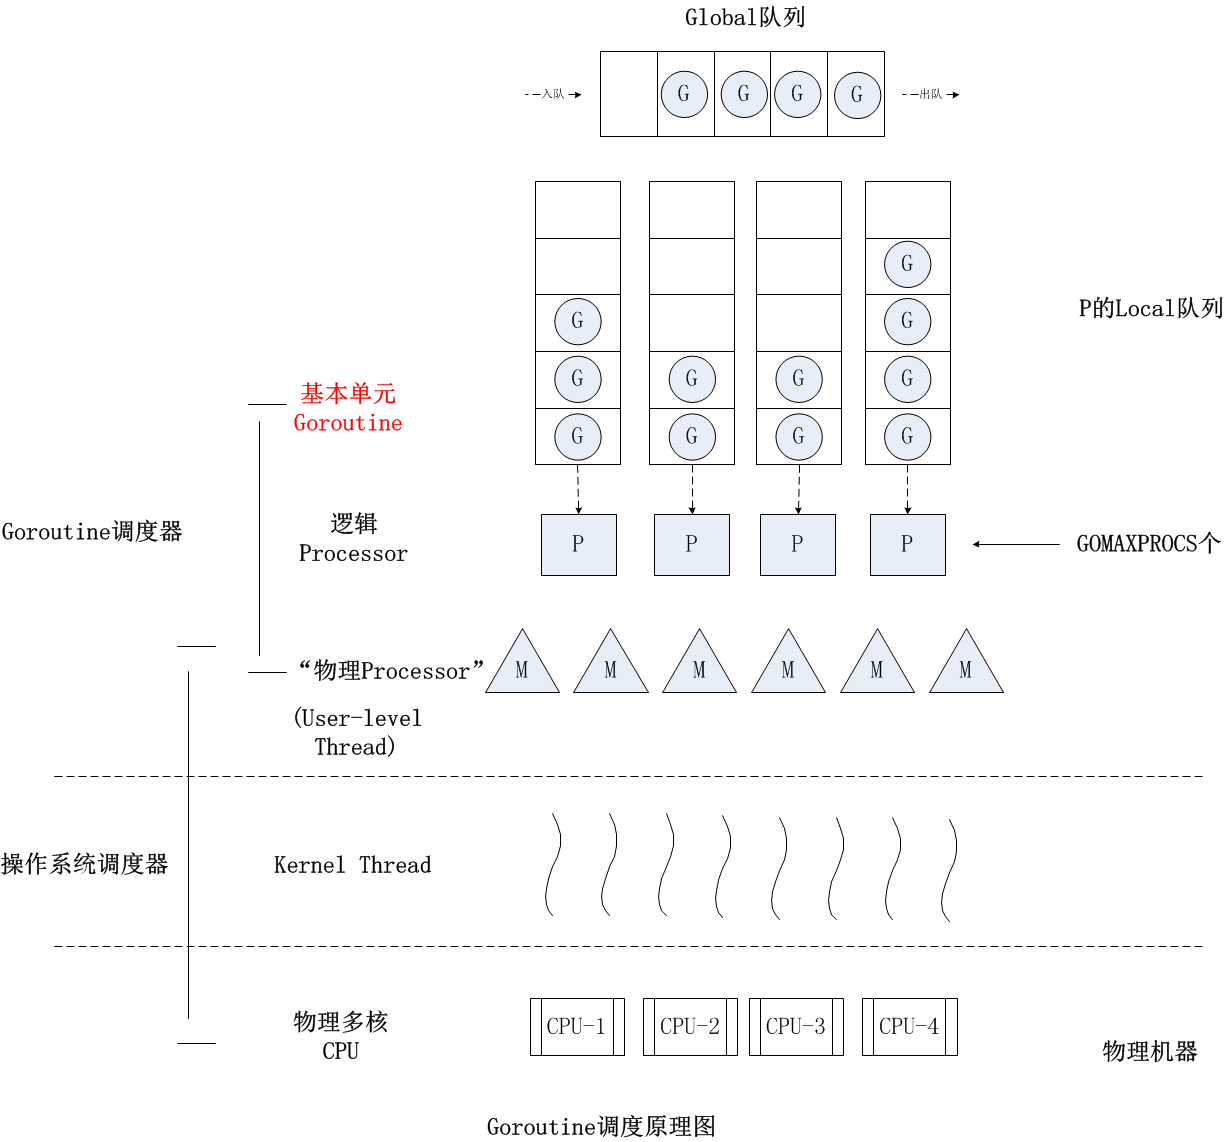
\includegraphics[width=.9\linewidth]{./goroutine.png}
\end{center}

    M 代表 OS 的线程,P 代表当前系统的处理器数( \texttt{runtime} 会检测当前处理器核数,这个是并行的前提,也是最大并行的能力),G 代表 \texttt{Golang} 语言的用户级线程,也就是通常所说的 \texttt{goroutine} 。
M 必须与 P 绑定方能执行任务 G。

从架构上来看,何其像 \texttt{Nginx} 的多进程+线程池模型。:)

从实现上来看, \texttt{goroutine} 在创建上为了性能也实现了线程池的复用特性(协程池)。

    从调度策略来看, \texttt{Golang} 完全是协作式调度,一个执行中的 \texttt{goroutine} 仅在操作被阻塞或显示让出处理器时被切换出去, \texttt{goroutine} 之间也没有优先级之分。
值得注意的是在 \texttt{Golang} 1.2 版之后,增加了一些简单的抢占机制,但仅有用户程序函数调用时刻才可能触发抢占的判断,并不是真正意义上的抢占。

\subsubsection{\texttt{Golang} 并发同步}
\label{sec:org9b6cff8}
在多线程编程中,我们一定会遇到数据竞态问题,这个时候我们需要一种锁机制来同步竞态数据。比较常规的手段有互斥对象、条件变量、原子操作,内存序等等。但在多线程编程中无锁编程一直是我们孜孜不倦的追求。
\texttt{Golang} 给我们提供一种外观上的无锁同步机制 -- \texttt{Channel} ,类似于 \texttt{Unix} 的管道。

\texttt{Channel} 的底层结构:
\lstset{language=go,label= ,caption= ,captionpos=b,numbers=none}
\begin{lstlisting}
type hchan struct {
    qcount   uint           // total data in the queue
    dataqsiz uint           // size of the circular queue
    buf      unsafe.Pointer // points to an array of dataqsiz elements
    elemsize uint16
    closed   uint32
    elemtype *_type // element type
    sendx    uint   // send index
    recvx    uint   // receive index
    recvq    waitq  // list of recv waiters
    sendq    waitq  // list of send waiters

    // lock protects all fields in hchan, as well as several
    // fields in sudogs blocked on this channel.
    //
    // Do not change another G's status while holding this lock
    // (in particular, do not ready a G), as this can deadlock
    // with stack shrinking.
    lock mutex
}
\end{lstlisting}

\texttt{Channel} 的声明方式:
\lstset{language=go,label= ,caption= ,captionpos=b,numbers=none}
\begin{lstlisting}
ChannelType = ( "chan" | "chan" "<-" | "<-" "chan" ) ElementType .
\end{lstlisting}

在使用 \texttt{Golang} 并发编程的时候有这么一条要求: \textbf{不要通过共享内存来通信,而应该通过通信来共享内存} 。这个通信的重担主要是在 \texttt{Channel} 身上。
\lstset{language=go,label= ,caption= ,captionpos=b,numbers=none}
\begin{lstlisting}
package main

import (
    "fmt"
    "sync"
)

func main() {
    ch := make(chan int64) //非缓冲性,主要用于竞态数据同步
    ch2 := make(chan int64, 3) //缓冲性,主要用于消息传递

    go func() {
        ch <- int64(4)
    }()

    go func() {
        for i := 0; i < 3; i++ {
            ch2 <- int64(i)
        }
    }()

    var wg sync.WaitGroup
    go func() {
        wg.Add(1)
        for i := 0; i < 3; i++ {
            v := <-ch2
            fmt.Println(v)
        }
        wg.Done()
    }()

    fmt.Println(<-ch)
    wg.Wait()
}
\end{lstlisting}

\subsubsection{C++20 的协程实现方式}
\label{sec:orgd740b2f}
\texttt{C++} 的协程实现方式是非对称式,第一类级,无栈式。底层实现为线程池。C++20 的协程可能实现如下图:

\begin{center}
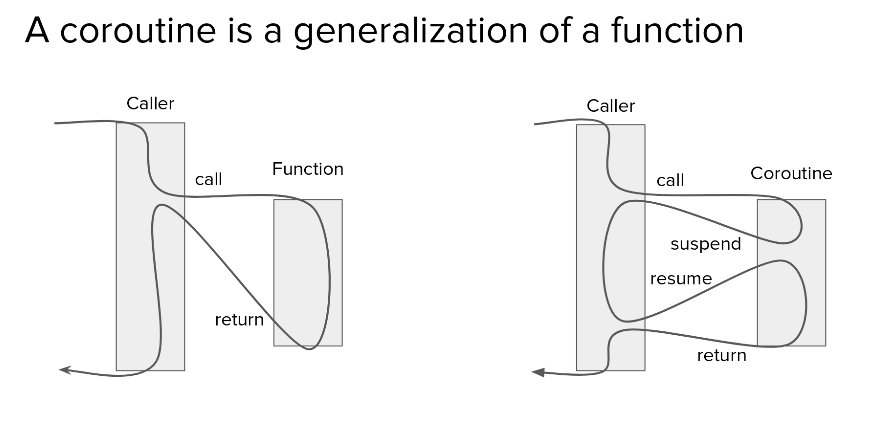
\includegraphics[width=.9\linewidth]{./coroutine.png}
\end{center}

\section{参考文档}
\label{sec:orga25c1f4}

\begin{itemize}
\item \href{https://www.amazon.cn/\%E6\%93\%8D\%E4\%BD\%9C\%E7\%B3\%BB\%E7\%BB\%9F\%E6\%A6\%82\%E5\%BF\%B5-\%E8\%A5\%BF\%E5\%B0\%94\%E4\%BC\%AF\%E6\%9F\%A5\%E8\%8C\%A8/dp/B004OQE8BI/ref=sr\_1\_1?ie=UTF8\&qid=1509954065\&sr=8-1\&keywords=\%E6\%93\%8D\%E4\%BD\%9C\%E7\%B3\%BB\%E7\%BB\%9F\%E6\%A6\%82\%E5\%BF\%B5}{操作系统概念(第 7 版)}

\item \href{http://llvm.org/docs/Coroutines.html}{Coroutines in LLVM}

\item \href{https://github.com/qyuhen/book/blob/master/Go\%201.5\%20\%E6\%BA\%90\%E7\%A0\%81\%E5\%89\%96\%E6\%9E\%90\%20\%EF\%BC\%88\%E4\%B9\%A6\%E7\%AD\%BE\%E7\%89\%88\%EF\%BC\%89.pdf}{Go 1.5 源码剖析}

\item \href{http://www.modernescpp.com/index.php/coroutines}{C++20 Coroutines}

\item \href{https://github.com/k2huang/blogpost/blob/master/golang/\%E5\%B9\%B6\%E5\%8F\%91\%E7\%BC\%96\%E7\%A8\%8B/\%E5\%B9\%B6\%E5\%8F\%91\%E6\%9C\%BA\%E5\%88\%B6/Go\%E5\%B9\%B6\%E5\%8F\%91\%E6\%9C\%BA\%E5\%88\%B6.md}{Go 并发机制}
\end{itemize}
\end{document}